\documentclass[a4paper,8pt]{article} % a4, 8pt, article
\usepackage{geometry} % papersize
\geometry { % paper type + spacing
	a4paper,
	top=2cm,
	bottom=2.5cm,
	left=2cm,
	right=2cm
}
\usepackage{fancyhdr} % headers
\usepackage[german]{babel} % language
\usepackage[utf8]{inputenc} % lovely utf-8
\usepackage{graphicx} % images
\usepackage{wrapfig} % images
\usepackage{array} % allways use this shit, idk why
\usepackage{tikz} % draw stuff
\usepackage{ifthen} % draw stuff
\usetikzlibrary{shapes,calc,fadings} % draw stuff
\usepackage{xspace} % usefull idk, allways import this stuff
\usepackage{dirtytalk} % \say because fuck it
\usepackage{setspace} % don't ask, kind of like it...
\usepackage{pgfplots} % graphs
\usepackage{lastpage} % for the pagenumber
\usepackage{titlesec} % to change title size

%smaller sections, subsections, subsubsections, paragraphs and subparagraphs
\titleformat*{\section}{\normalsize\bfseries}
\titleformat*{\subsection}{\small\bfseries}
\titleformat*{\subsubsection}{\small\bfseries}
\titleformat*{\paragraph}{\small\bfseries}
\titleformat*{\subparagraph}{\small\bfseries}

\singlespacing % reduce spaceing

\graphicspath{ {./images/} }

\def \license {GNU Free Documentation License} % gpl for the win
\author{Sven Hugi} % author(s)

%\makeatletter % to use \@
% header and footer with fancy
\pagestyle{fancy} % set pagestyle
\fancyhf{} % just do it -> fancy think it's fancy to do so...
\rhead{Gibb M153} % right header
\lhead{Test 1, AB 1 - 4} % left header
\chead{inf-2018i} % center header
\cfoot{\thepage/\pageref{LastPage}} % center footer -> pagenmbr
\lfoot{License: \license} % left footer

% highlighting with some random effect -> looks handmade and i love it...
\newcommand\hl[2][yellow]{
	\begin{tikzpicture}[
		baseline,
		decoration={random steps,amplitude=0.5pt,segment length=5pt},
		outer sep=-5pt, inner sep = 0pt
		]
		\node[decorate,rectangle,fill=#1,anchor=text]{#2\xspace};
	\end{tikzpicture}
}
\makeatother % don't touch
%%%%%%%%%%%%%%%%%%%%%%%%%%%%%%%%%%%%%%%%%%%%%%%%%%%%%%%%%%%%%%%%%%%%%%%%%%%%%%%%%%%%%%%%%%%%%%%%%%%%%%%%%%%%%%%%%%%%%%%%%%%%%%%%%
%											Begin with the fucking document														%
%%%%%%%%%%%%%%%%%%%%%%%%%%%%%%%%%%%%%%%%%%%%%%%%%%%%%%%%%%%%%%%%%%%%%%%%%%%%%%%%%%%%%%%%%%%%%%%%%%%%%%%%%%%%%%%%%%%%%%%%%%%%%%%%%
\begin{document}
	\begin{small}
	\section{SQL}
		\begin{tabular}{m{2cm}|p{14.25cm}}
			Command 		& Description\\\hline\hline
			USE				& wechselt den Ausführungskontext auf eine bestimmte Datenbank. \hl{USE master}, in diesem Fall wird zur \hl[green]{Metadaten DB} gewechselt.\\\hline
			SELECT			& \hl[pink]{SELECT [Collumn name] FROM [Table name]}\\\hline
			UPDATE			& \hl[pink]{UPDATE [Table name] SET [collumn name] = [value], ... WHERE [condition]}\\\hline
			DELETE			& \hl[pink]{DELETE FROM [Table name] WHERE [condition]}\\\hline
			INSERT INTO		& \hl[pink]{INSERT INTO [Table name] ([column1, column2,...]) VALUES ([value1, value2,...])}\\\hline
			GO				& wird verwendet, um die Ausführung zu erzwingen.\\\hline
			CREATE DATABASE	& kreiert eine neue Datenbank, zu welcher man mit \hl{USE} wechseln kann\\\hline
			DROP DATABASE	& schmeisst die Datenbank aus dem Fenster\\\hline
			ON				& gibt an, wo die Daten physisch gespeichert werden.\\\hline
			CREATE TABLE	& um eine Tabele zu kreieren, \hl[pink]{CREATE TABLE [table name] ([Coll1, coll2 etc])}\\\hline
			DROP TABLE		& schmeisst die Table aus dem Fenster\\\hline
			ALTER TABLE		& \hl[pink]{ALTER TABLE [Table name] [DROP / ALTER] COLUMN [column name] [datatype (only if ALTER)]}\\\hline
			CONSTRAINT		& bedingung $\rightarrow$ z.B Key \hl[pink]{CONSTRAINT [key name] PRIMARY KEY  [type (optional)] ([referenz])} bzw \hl[pink]{CONSTRAINT [key name] FOREIGN KEY ([target]) REFERENCES}\hl[pink]{ [tabelle]([spallte])}\\\hline
			CREATE INDEX	& \hl[pink]{CREATE [type] INDEX [index name] ON [table] ([spallte])} man kann dann mit \hl{INCLUDE} andere Spallten includen.\\\hline
			DROP INDEX		& schmeisst den Index zum Fenster raus			
		\end{tabular}
		\begin{minipage}{0.5\linewidth}
			\section{Data Type}
			\begin{tabular}{c|c}
				Data type								& use\\\hline\hline
				bigint									& 64 bit number\\\hline
				\hl[green]{int}							& 32 bit number\\\hline
				smallint								& 16 bit number\\\hline
				\hl[green]{tinyint}						& 8 bit number\\\hline
				bit										& 1 bit number\\\hline
				\hl[green]{decimal(precision, scale)}	& floating point number\\\hline
				numeric									& same as decimal\\\hline
				money									& 64 bit int shifted\\\hline
				smallmoney								& 32 bit int shifted\\\hline
				float(n)								& float 1 - 24\\\hline
				\hl[green]{real}						& float(24)\\\hline
				\hl[green]{datetime}					& date and time 3ms\\\hline
				smalldatetime							& date and time 1min\\\hline
				char									& char max 8000\\\hline
				\hl[green]{varchar(n)}					& use this instead of char\\\hline
				nchar									& char in unicode\\\hline
				nvarchar(n)								& varchar in unicode\\\hline
				\hl[green]{text}						& long texts\\\hline
				ntext									& unicode text\\\hline
				binary									& malware\\\hline
				\hl[green]{varbinary(n)}				& use this instead of binary\\\hline
				\hl[green]{image}						& binary, but longer\\\hline
				cursor									& reference as cursor\\\hline
				sql\_variant							& never use this\\\hline
				table									& query result for later usage\\\hline
				timestamp								& timestamp\\\hline
				uniqueidentifier						& GUID\\\hline
			\end{tabular}
		\end{minipage}
		\begin{minipage}{0.5\linewidth}
			\section{Indexes}
				\begin{itemize}
					\item NONCLUSTERED
					\item CLUSTERED
				\end{itemize}
			 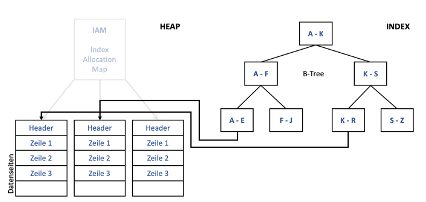
\includegraphics[width=.9\linewidth]{index}
			 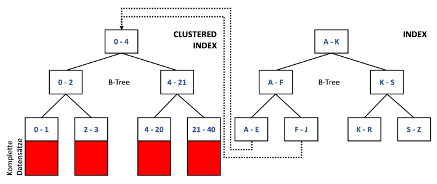
\includegraphics[width=.9\linewidth]{clusteredIndex}
			 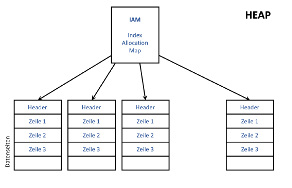
\includegraphics[width=.9\linewidth]{heap}
		\end{minipage}
	\section{binary search tree and b-tree}
		\begin{tikzpicture}
		\begin{scope}[
		level 1/.style={
			level distance=5mm,sibling distance=12mm
		},
		level 2/.style={
			level distance=5mm,sibling distance=8mm
		},
		level 3/.style={
			level distance=5mm,sibling distance=8mm
		},
		font=\tiny,inner sep=0.5pt,every node/.style={
			draw,circle,minimum size=10pt
		}
		]
		\node {51} % root
		child {
			node {22} % lvl 1
			child {
				node{1} % lvl 2
			} 
			child {
				node{42} % lvl 3
				child {
					node{37}
				} 
				child[missing]
			}
			edge from parent
		}
		child {
			node {87} % lvl 1
			child {
				node {52} % lvl 2
				child[missing]
				child {
					node{86} % lvl 3
				}
			}
			child {
				node {94}
			}
		};
		\end{scope}
		\begin{scope}[xshift=0.25\linewidth,
		level 1/.style={
			level distance=5mm,sibling distance=8mm
		},
		font=\tiny,
		inner sep=2pt,
		every node/.style={
			rectangle split, rectangle split horizontal,rectangle split ignore empty parts,draw
		}
		]
		\node {2 \nodepart{two} 4}
		child {
			node {1}
		}
		child {
			node {3}
		}
		child {
			node {5}
		};
		
		\end{scope}
		\begin{scope}[xshift=0.5\linewidth,
		level 1/.style={
			level distance=5mm,sibling distance=8mm
		},
		font=\tiny,
		inner sep=2pt,
		every node/.style={
			rectangle split, rectangle split horizontal,rectangle split ignore empty parts,draw
		}
		]
		\node {2 \nodepart{two} 4}
		child {
			node {1}
		}
		child {
			node {3}
		}
		child {
			node {5 \nodepart{two} 6}
		};
			
		\end{scope}
		\begin{scope}[xshift=0.75\linewidth,
		level 1/.style={
			level distance=5mm,sibling distance=16mm
		},
		level 2/.style={
			level distance=5mm,sibling distance=8mm
		},
		font=\tiny,
		inner sep=2pt,
		every node/.style={
			rectangle split, rectangle split horizontal,rectangle split ignore empty parts,draw
		}
		]
		
		\node {4 \nodepart{two}}
		child {
			node {2}
			child {
				node{1}
			}
			child {
				node{3}
			}
		}
		child {
			node{6}
			child {
				node{5}
			}
			child {
				node{7}
			}
		};
		\end{scope}
		\end{tikzpicture}
.\linebreak
	\begin{minipage}{0.68 \linewidth}
		\subsection{b-tree ersparrniss}
		$maximale Schritte\ =\ \frac{
			\log_{10} (n)
		}{
			\log_{10} (Anzahl Verzweigungen)
		}\ vs\ Heap\ n \rightarrow \emptyset\ \frac{n}{2}$
		\section{DM}
			\begin{tabular}{c|c|c|c}
				Element					&Voranalyse	&Konzeptionelles DM	&Logisches DM\\\hline\hline
				Entitäten Namen			&X			&X					&\\\hline
				Entitäten Beziehungen	&X			&X					&\\\hline
				Attribute Namen			&			&X					&\\\hline
				Primärschlüssel			&			&X					&X\\\hline
				Fremdschlüssel			&			&					&X\\\hline
				Tabellen Namen			&			&					&X\\\hline
				Spalten Namen			&			&					&X\\\hline
				Datentypen				&			&					&X\\\hline
			\end{tabular}
			\section{4 Fälle}
			\begin{itemize}
				\item überlappend (X kann auch Y sein)
				\item disjunkt (X kann nicht auch Y sein)
				\item total (jedes X muss auch zu Y gehören)
				\item partiell (X muss nicht unbedint zu Y gehören)
			\end{itemize}
	\section{Beziehungen}
		\subsection{Hierarchisch}
			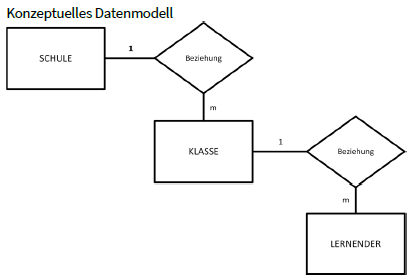
\includegraphics[width=.5\linewidth]{hierarchie}
			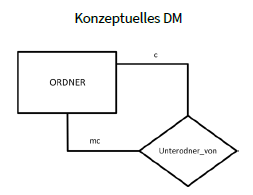
\includegraphics[width=.5\linewidth]{hierarchie2}
		\subsection{Netzwerkartig}
			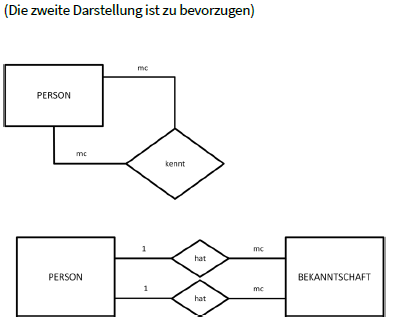
\includegraphics[width=.5\linewidth]{network}
	\end{minipage}
	\begin{minipage}{0.32 \linewidth}
		\section{Spezialisierung / Generalisierung}
			\begin{itemize}
				\item \hl[green]{Superklasse und Subklasse je}\hl[green]{eine Tabelle(bekannt)}
				\item Eine Klasse pro Subklasse(keine Superklasse)
				\item Alles in einer Tabelle1 zusätzliches Attribut
				\item Alles in einer Tabelle mit 1 zusätzlichen Attribut pro Subklasse
			\end{itemize}
			\subsection{Spezialisierung}
				Top Down Sicht, ein in mehrere aufteilen.
			\subsection{Generalisierung}
				Bottom Up Sicht, mehrere zusammenfassen.
		\section{Diagramm}
			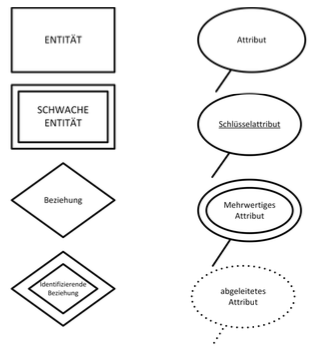
\includegraphics[width=\linewidth]{diagramm}
			\linebreak
			- \hl[green]{UML}\\
			- Nur Attribut namen in Tabelle\\
			- Alle Details in Tabelle
			\subsection{TADESI}
			\begin{tabular}{c|c}
				T	& Tabellenname\\\hline
				A	& Attribute\\\hline
				D	& Datentypen\\\hline
				E	& Constraints (NULL, DEAFULT)\\\hline
				S	& Schlüsselarten (PK, FK)\\\hline
				I	& Indexe\\
			\end{tabular}
	\end{minipage}
	\end{small}
\end{document}